\chapter{DL\,07 – Regression: Zahlenwerte vorhersagen (optional)}

\begin{myremark}
Diese Doppellektion ist \textbf{optional}. Sie setzt DL\,01--02 voraus.
Regression erweitert das Konzept aus DL\,01 (\enquote{Prediction}) und zeigt,
wie kontinuierliche Ausgabewerte modelliert werden.
\end{myremark}

\section{Lineare Regression}

\begin{mydefinition}[Lineare Regression]
Die \textbf{lineare Regression} sagt einen kontinuierlichen Zahlenwert $y$ auf Basis
von Merkmalen $x_1, x_2, \ldots, x_n$ vorher:
\[
y = a_0 + a_1 x_1 + a_2 x_2 + \cdots + a_n x_n
\]
Die Koeffizienten $a_i$ werden durch \textbf{Minimierung des quadratischen Fehlers} bestimmt
(Methode der kleinsten Quadrate).
\end{mydefinition}

\begin{figure}[H]
    \centering
    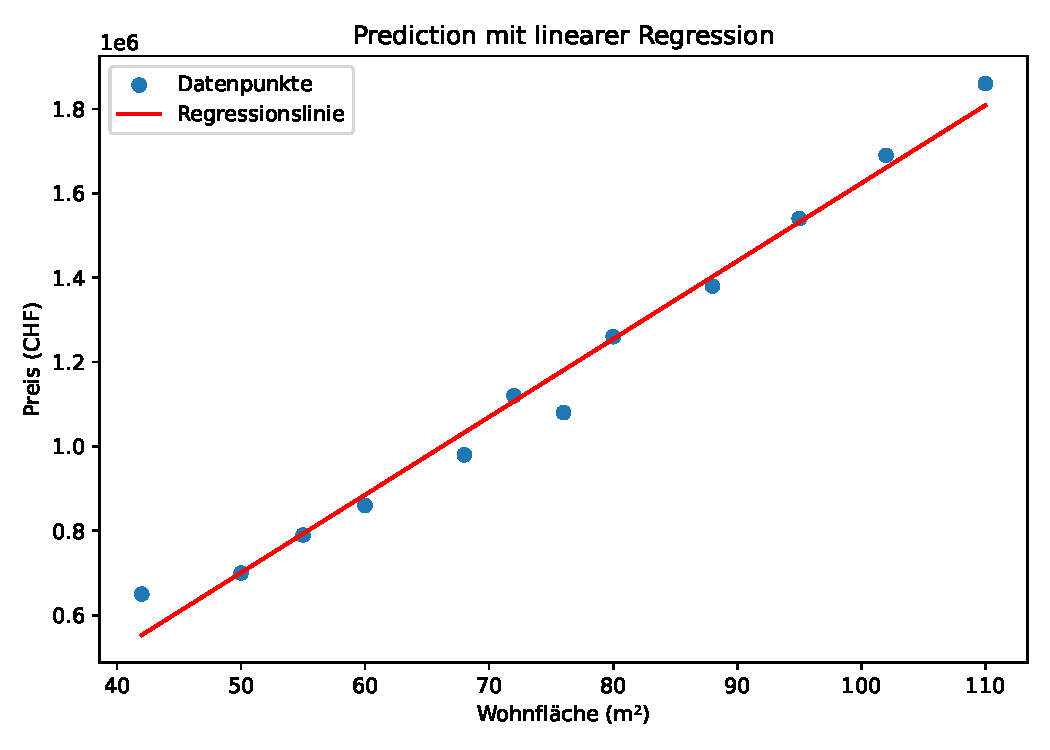
\includegraphics[width=0.75\textwidth]{Grundlagen_Info/15_KI_und_Algorithmen/Figures/regression_prediction.pdf}
    \caption{Lineare Regression: Vorhersage der Wohnungsmiete in Abhängigkeit der Wohnfläche}
    \label{fig:reg-pred-15}
\end{figure}

\section{Interpretation der Koeffizienten}

\begin{myexercise}[Koeffizienten interpretieren]
Ein Regressionsmodell für Wohnungsmieten lautet:
\[
\hat{y} = 500 + 8 \cdot \text{Fläche} - 30 \cdot \text{Stockwerk}
\]
\begin{enumerate}
    \item Was bedeutet der Koeffizient $8$ für die Fläche inhaltlich?
    \item Was bedeutet $-30$ für das Stockwerk? Ist das plausibel?
    \item Wie hoch ist die Vorhersage für eine 60\,m\textsuperscript{2}-Wohnung im 3.\,Stockwerk?
\end{enumerate}
\begin{myanswer}
1.\ Pro m\textsuperscript{2} mehr steigt die Miete um CHF\,8. \\
2.\ Pro Stockwerk höher sinkt die Miete um CHF\,30 (weniger plausibel, eher Datenproblem). \\
3.\ $\hat{y} = 500 + 8 \cdot 60 - 30 \cdot 3 = 500 + 480 - 90 = 890$ CHF.
\end{myanswer}
\end{myexercise}

\section{Gütemasse für Regression}

\begin{mydefinition}[MAE und RMSE]
\[
\text{MAE} = \frac{1}{n}\sum_{i=1}^{n} |y_i - \hat{y}_i|
\qquad\qquad
\text{RMSE} = \sqrt{\frac{1}{n}\sum_{i=1}^{n} (y_i - \hat{y}_i)^2}
\]
\end{mydefinition}

\begin{myexercise}[Fehlermasse vergleichen]
\begin{enumerate}
    \item Welches Mass bestraft grosse Einzelfehler stärker – MAE oder RMSE?
    \item In welchem Anwendungsfall wäre RMSE besonders sinnvoll?
\end{enumerate}
\begin{myanswer}
1.\ RMSE, weil die Fehler quadriert werden. \\
2.\ Wenn einzelne Ausreisser besonders kritisch sind, z.\,B. bei Energieprognosen für Spitzenlast.
\end{myanswer}
\end{myexercise}

\section{Grenzen der linearen Regression}

\begin{mycaution}
Lineare Regression kann nur \textbf{lineare Zusammenhänge} abbilden.
Bei nichtlinearen Beziehungen (z.\,B. exponentielles Wachstum) sind Erweiterungen wie
\textbf{polynomiale Regression} oder \textbf{Entscheidungsbäume für Regression} nötig.
\end{mycaution}

\begin{mychallenge}[Nichtlineare Daten]
Laden Sie den Datensatz \texttt{apartment\_prices.csv} und fügen Sie ein quadratisches
Feature $\text{Fläche}^2$ hinzu (\emph{Polynomial Features}).
\begin{itemize}
    \item Vergleichen Sie RMSE des linearen und des polynomialen Modells.
    \item Ab welchem Polynomgrad zeigt sich Overfitting?
\end{itemize}
\end{mychallenge}

\begin{myremark}[Notebook]
Praktische Umsetzung inkl. Übungen:
\href{\notebookbaseurl05_Regression_Prediction.ipynb}{\texttt{05\_Regression\_Prediction.ipynb}}
\end{myremark}
